\chapter{Architektur}


\section{Equalizer}

\subsection{Equalizer Prozesse}

Equalizer ist auf dem Client-Server Modell aufgebaut. Eine vereinfachte Darstellung der Architektur ist in Abbildung \ref{eq_proc} ersichtlich.

\begin{description}
\item[Equalizer Server] Der Server ist f\"ur das Management eines einzelnen Visualisierungssystems zust\"andig. Er startet die Rendering Clients der Applikation.
\item[Application] Die Applikation ist das Herzst\"uck. Beim Starten der Applikation verbindet sich diese zum Equalizer Server, welcher daraufhin eine Konfiguration schickt. Die Applikation verarbeitet ausserdem Events und kontrolliert das Rendering ihrer Clients.
\item[Application Render Client] Der Render Client implementiert den Rendering Teil der Applikation. Es gibt keinen Main-Loop in der Ausf\"uhrung, alle Tasks werden vom Server gesteuert.
\end{description}

\begin{figure}[ht]
\centering
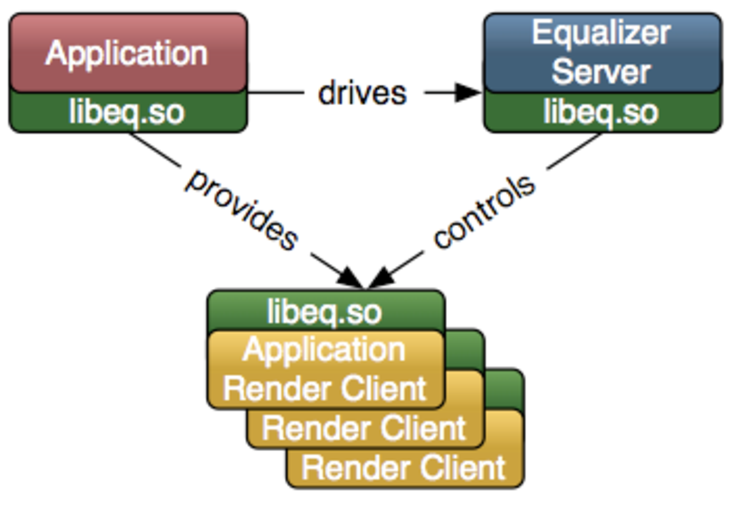
\includegraphics[scale=0.5]{../figures/equalizer_model}
\caption{Equalizer Prozesse, (Quelle: [1, Seite 2])}
\label{eq_proc}
\end{figure}

Abbildung \ref{eq_exec} zeigt ein vereinfachtes Modell eines Execution Models. Equalizer kreiert f\"ur jede verwendete Grafikkarte einen einzelnen Thread. Die Threads werden asynchron zueinander ausgef\"uhrt.

\begin{figure}[ht]
\centering
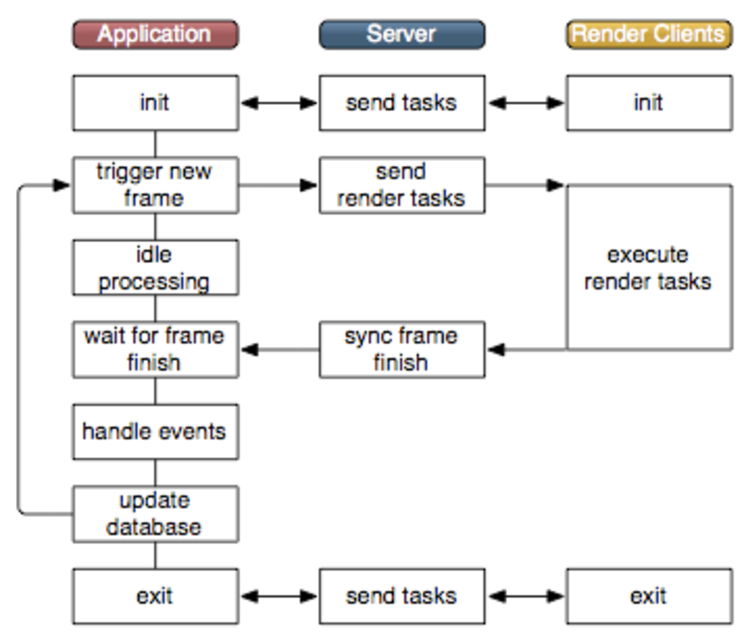
\includegraphics[scale=0.5]{../figures/equalizer_execution_flow}
\caption{Equalizer Execution Model, (Quelle [1, Seite 9])}
\label{eq_exec}
\end{figure}

\subsection{Stereo}
Wie bereits in einem fr\"uheren Kapitel beschrieben, unterst\"utzt Equalizer Stereo Compounds. Bei Stereo Compounds wird f\"ur jedes Auge eine separate Rendering Unit verwendet. Die Bilder werden nach dem Rendern in einen Stereobuffer gespeichert. 


\subsection{Config}
Die Konfiguration einer Equalizer Applikation repr\"asentiert die Session, in der alle Render Clients registriert werden. Sie beinhaltet eine Beschreibung der Rendering Ressourcen und deren Verwendung. Diese werden in einer Baumstruktur aufgebaut, die der physikalischen Hierarchie einer 3D Rendering Umgebung entspricht. 
Abbildung \ref{eq_ex_config} zeigt eine Beispiel Konfiguration f\"ur einen 4-Wand CAVE. Die Applikation wird auf zwei Workstations (Nodes) mit drei Grafikkarten (Pipes) gerechnet. M\"ochte man dieselbe Applikation auf einer anderen Topologie rendern lassen, so reicht es also, die Konfiguration von Equalizer anzupassen.

\section{CAVE Rendering Framework}

\subsection{Grobarchitektur}
Das Hauptziel unserer Arbeit besteht darin, eine Verbindung zwischen einem SceneGraph und Equalizer herzustellen (Abbildung \ref{cave_arch}). Eine Studentengruppe aus Siegen, Deutschland, hat vor einiger Zeit mit einem \"ahnlichen Projekt angefangen - eqOSG. Sie haben dazu eine Beispiel Applikation entwickelt. Es gilt noch zu pr\"ufen, ob diese Implementation unseren Zwecken gen\"ugt, und ob wir darauf aufbauen k\"onnen.
Wichtig f\"ur das Framework unsererseits ist es, dass es flexibel ist gegen\"uber anderen VR Techniken wie zum Beispiel Haptics.

\begin{figure}[ht]
\centering
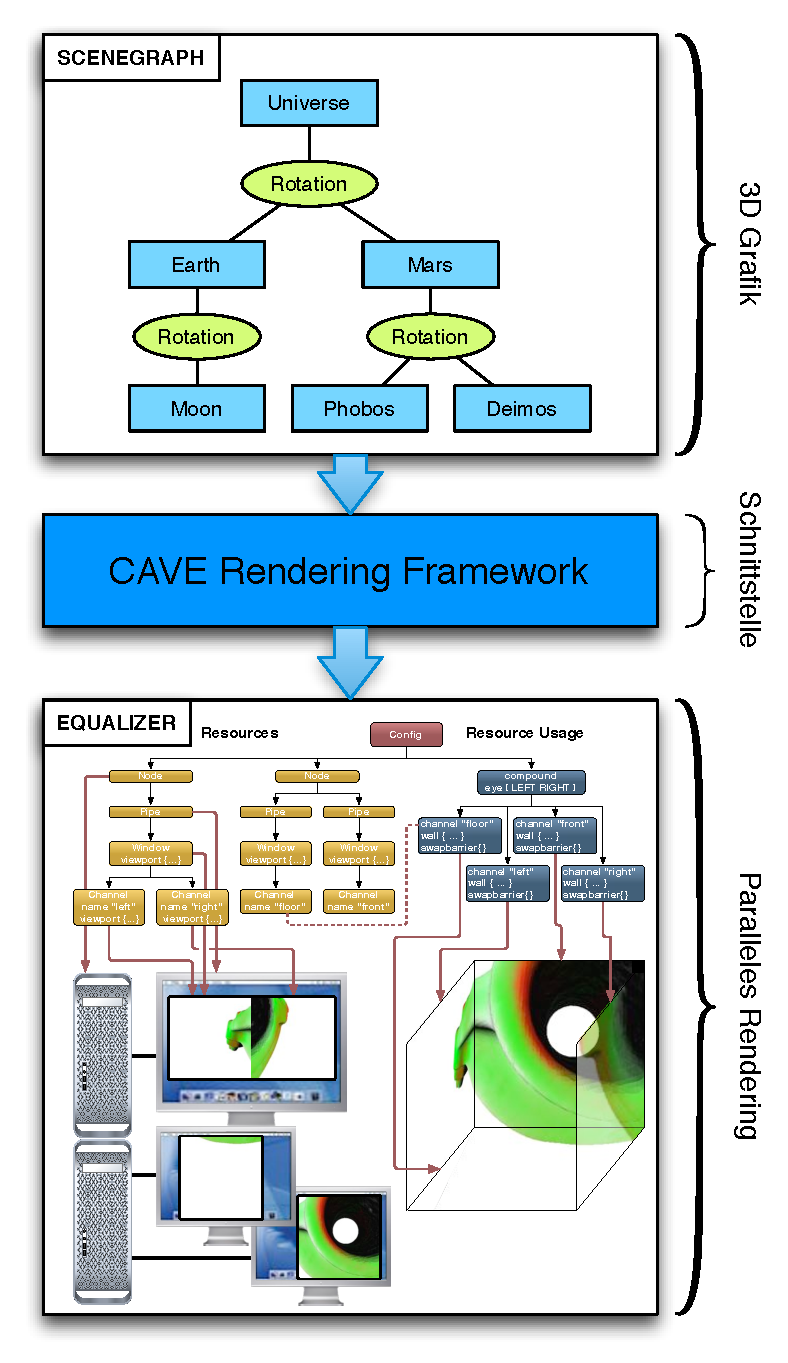
\includegraphics[scale=0.6]{../figures/crf_architecture_pflichtenheft}
\caption{CAVE Architektur}
\label{cave_arch}
\end{figure}

\subsection{eqOSG}
Wie bereits erw\"ahnt, wird an der Universit\"at Siegen, Deutschland, ebenfalls an einem Projekt gearbeitet, OpenSceneGraph in Equalizer zu integrieren. 
Equalizer stellt ein Interface von Klassen zur Verf\"ugung um Applikationen zu entwickeln. Abbildung \ref{pack_mod} zeigt die Grobstruktur einer Implementation. Wie man sieht, gibt es in Equalizer ein Paket \texttt{eq} mit den Hauptklassen. 

\begin{figure}[ht]
\centering
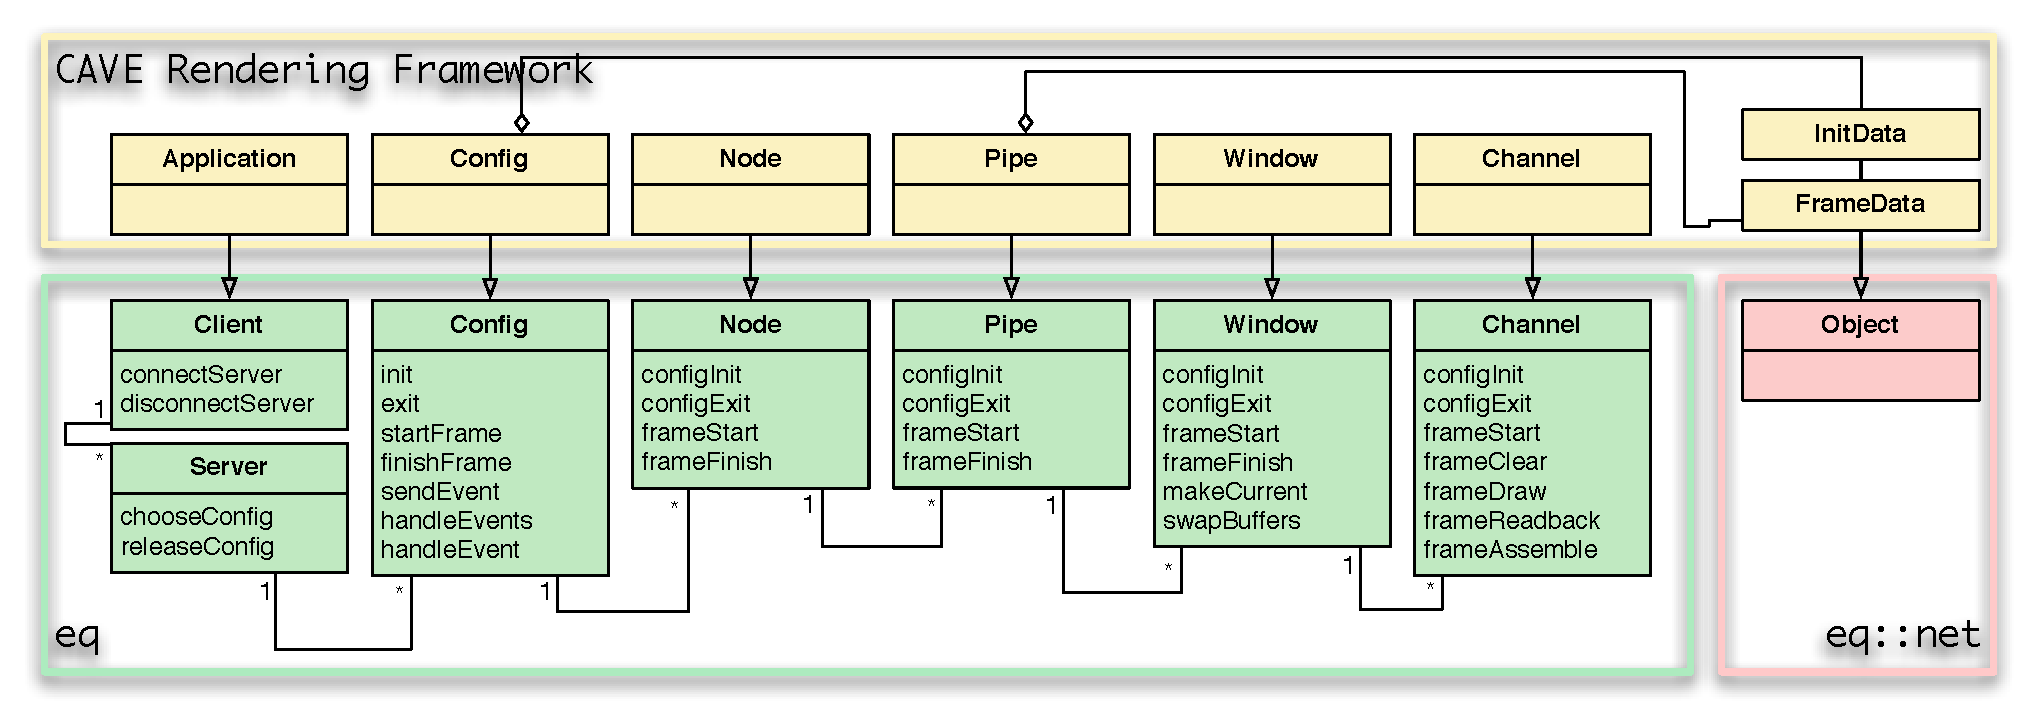
\includegraphics[scale=0.4]{../figures/crf_namespaces}
\caption{Package Modul}
\label{pack_mod}
\end{figure}

\subsection{CAVE Konfigurationen}
Wie in Abschnitt \ref{sg_eq_int} beschrieben, soll Equalizer so konfigurierbar sein, dass das Rendering mit verschiedenen Topologien m\"oglich ist. Dabei sollte es m\"oglich sein, dem Entwickler ein Interface zu bieten, bei dem er sich nicht um Konfigurationen k\"ummern muss, ausser er will eine neue Topologie aufbauen.

Das Design Pattern \textit{Facade} bietet sich daf\"ur an. Bei diesem Pattern handelt es sich um ein Structural Pattern. Es bietet eine einheitliche Schnittstelle zu einer Menge von Schnittstellen eines Subsystems, in unserem Fall die verschiedenen Konfigurationen der VR-Systeme.
Ein Subsystem wie es Equalizer darstellt, beinhaltet viele technisch orientierte Klassen, die von aussen selten oder nie gebraucht werden. Ein Entwickler braucht meist keine Informationen \"uber die verschiedenen Nodes und Pipes zu haben. Die Fassade ist eine Klasse mit ausgew\"ahlten Methoden, die eine h\"aufig ben\"otigte Untermenge an Funktionalit\"at des Subsystems umfasst. Sie delegiert die Funktionalit\"at an andere Klassen des Subsystems und vereinfacht dadurch den Umgang mit dem System.


\begin{figure}[ht]
\centering
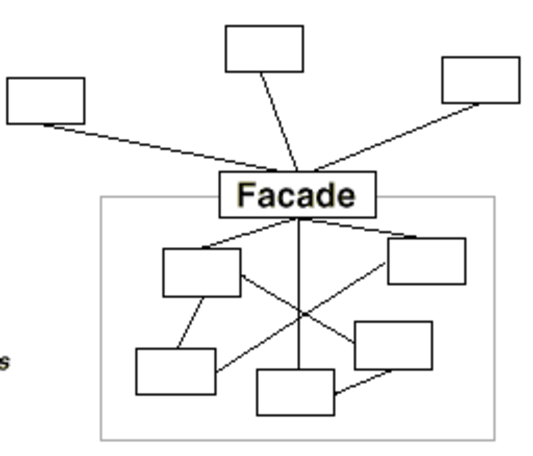
\includegraphics[scale=0.5]{../figures/facade_pattern}
\caption{Facade Pattern (Quelle: [3])}
\end{figure}
